\documentclass[11pt]{article}
\usepackage[margin=2.2cm]{geometry}
\usepackage[T1]{fontenc}
\usepackage{amsmath,amssymb,booktabs,graphicx,xcolor,enumitem,caption,float,longtable}
\usepackage{hyperref}
\setlist{itemsep=2pt,topsep=3pt}
\hypersetup{colorlinks=true,linkcolor=blue!50!black,urlcolor=blue!50!black}
\captionsetup{font=small,labelfont=bf}
\setlength{\emergencystretch}{3em}
\setlength{\parskip}{4pt}
% every figure sits where its text is ([H]); the text about a figure comes right before it
\newcommand{\fig}[2]{\begin{figure}[H]\centering\includegraphics[width=\textwidth]{figures/#1}\caption{#2}\end{figure}}
\newcommand{\takeaway}[1]{\par\noindent\fcolorbox{gray!50}{gray!8}{\parbox{\dimexpr\textwidth-2\fboxsep-2\fboxrule}{\textbf{Take-away.} #1}}\par\medskip}

\title{v3: what the voltages do to noise, dark charge and gain,\\ and how well the models see it}
\author{ccd\_opt\_ml}
\date{2026-11-16}

\begin{document}
\maketitle

\section*{Summary}
\begin{enumerate}
\item \textbf{What the voltages do.} With the timing fixed, \textbf{VSUB} sets the dark charge ($\lambda$ +34\,\% per SD,
  96\,\% of its variance) and most of the noise ($\sigma_e$ +4.9\,\%/SD, steep above $\approx$55\,V). \textbf{VDD and VR} set
  the gain ($-1.6$ and $-2.1$\,\%/V). Every other voltage moves $\sigma_e$ by 1--1.5\,\%/SD and $\lambda$ by 2--5\,\%/SD:
  SW low, VDD, VR, RG high/low, V1 low, the H highs.
\item \textbf{Correlations mislead for the clock rails.} The V lows and H3 rails look tied to noise and dark charge
  ($|r|$ up to 0.37); with the other voltages held fixed they are not ($\le0.11$): the relational rules made them move
  with VSUB.
\item \textbf{Models.} $\lambda$ and gain changes are a ``settings'' problem ($\rho$ 0.87--0.93 on a new amplifier);
  adding the traces cuts the $\lambda$ change error from 36 to 25\,\%. $\sigma_e$ changes are hard for every model
  ($\rho\approx0.6$--0.7). The small effects (VSUB held): the settings still see $\lambda$ ($\rho$ 0.71), the traces see
  $\sigma_e$ slightly better than the settings (0.49 vs 0.43).
\item \textbf{Sealed test (session H, 24 new settings).} The frozen choice held: every frozen model kept or improved its
  rank correlation; errors grew by 1--3 points only because H's changes are larger (no-change baseline 14.0 vs 11.9\,\%
  for $\sigma_e$). One frozen trace model (difference curves PCA) did not carry over ($\rho$ 0.59 $\to$ 0.46).
\end{enumerate}


\paragraph{Words.} An \emph{image} (about 10 minutes) gives the true \textbf{noise} $\sigma_e$, \textbf{dark charge}
$\lambda$ and \textbf{gain}. A \emph{trace} is a fast (0.2\,s) recording of the amplifier output; its \emph{noise
components} (white noise, 1/f corner, Allan deviation, power in frequency bands) are measured from it.
An \emph{absolute} model predicts a value; a \emph{change} model predicts how much a value changes between two settings
of the same amplifier. A \emph{new amplifier} is one the model never saw in training. \emph{1 SD} of a voltage is its
standard deviation over the v3 packets (VSUB 9.8\,V, VDD 1.0\,V, RG low 1.1\,V, RG high 0.7\,V, SW low 0.6\,V, VR
0.5\,V, the H clock rails about 0.45\,V, the V clock rails 0.1--0.16\,V). Every effect is in \% because the outputs are
modelled in log units. $\rho$ is the rank (Spearman) correlation between predicted and true values: 1 = perfect order,
0 = no information.

\tableofcontents

% =====================================================================================================================
\section{The data}
The v3 noise set (\texttt{packet\_plan\_v3n}) holds the timing at nominal and varies only the voltages, each inside its
window, keeping the relational rules (every clock low at least 0.5\,V below its high, and so on). 127 packets on board
101, amplifiers ch0, ch1, ch3 (ch2 left out as before):
\begin{itemize}
\item \textbf{Session G (training):} 80 voltage settings drawn as a Sobol design (every packet moves every voltage), 14
  nominal packets (drift and label noise), 4 replicates. 232 usable measurements (packet $\times$ amplifier) after
  dropping three failed $\lambda$ fits at the fit floor.
\item \textbf{Session H (sealed test):} 24 new voltage settings + 5 nominal packets, scored \emph{once}, after the model
  choice was frozen (Section~\ref{sec:frozen}).
\end{itemize}
Repeated nominal packets give the measurement noise: $\sigma_e$ 1.0--1.6\,\%, $\lambda$ 2.9--4.4\,\%, gain 0.9\,\%
per image; for a \emph{change} between two images, $\sigma_e$ 1.9\,\%, $\lambda$ 12\,\%, gain 0.8\,\%. No model can do
better than that. The drift over the 49 hours is small ($\lambda$ +0.1 to +0.2\,\%/h).

Groups that always moved together are one knob: both SW lows, both RG highs, both RG lows, the A and B rails of V1,
V3, H1, H3, VDD1+2, VR1+2. TG stayed at nominal.

\paragraph{Did the voltages vary independently?} Mostly, but not completely. The relational rules tie each clock's
high to its low (H1, H2, H3 high vs low: $r\approx0.8$) and the V lows to SW low ($r\approx-0.65$), because a draw that
broke a rule was rejected. This matters for reading the effects: a ``high'' and a ``low'' of the same clock cannot be
fully told apart; their \emph{swing} (high $-$ low) can (Section~\ref{sec:swing}).
\fig{corr_design.png}{Design check: correlation between the voltages over the 94 session-G packets. 0 = varied
independently. The 0.8 blocks are each clock's high and low, tied by the relational rules.}

% =====================================================================================================================
\section{What every voltage does}\label{sec:effects}
Three views, all on session G, all with the amplifier offset removed:
\begin{enumerate}
\item \textbf{Effects} (Fig.~\ref{fig:effectmap}, Table~\ref{tab:effects}): a linear model with all voltages at once;
  \% change of the output per 1~SD of each voltage, with a 68\,\% bootstrap interval over the packets.
\item \textbf{Correlations} (Section~\ref{sec:corr}): plain and partial (``this voltage alone'').
\item \textbf{Shape} (partial dependence, Section~\ref{sec:shape}): boosted trees on all voltages; how the output
  moves along one voltage with the others averaged out. This shows thresholds and knees that a linear effect hides.
\end{enumerate}
The $R^2$ under each output says how much of its variation (within an amplifier) the voltages explain. Read an output's
column only when its $R^2$ is good: $\sigma_e$ 0.78, $\lambda$ 0.95, gain 0.87, trace white noise 0.87.
The 1/f corner ($R^2\approx0$), the slow/fast CDS power ratio (0.28) and the Allan deviation (0.41) are mostly
not set by the voltages, or too noisy per trace to tell.

\begin{figure}[H]\centering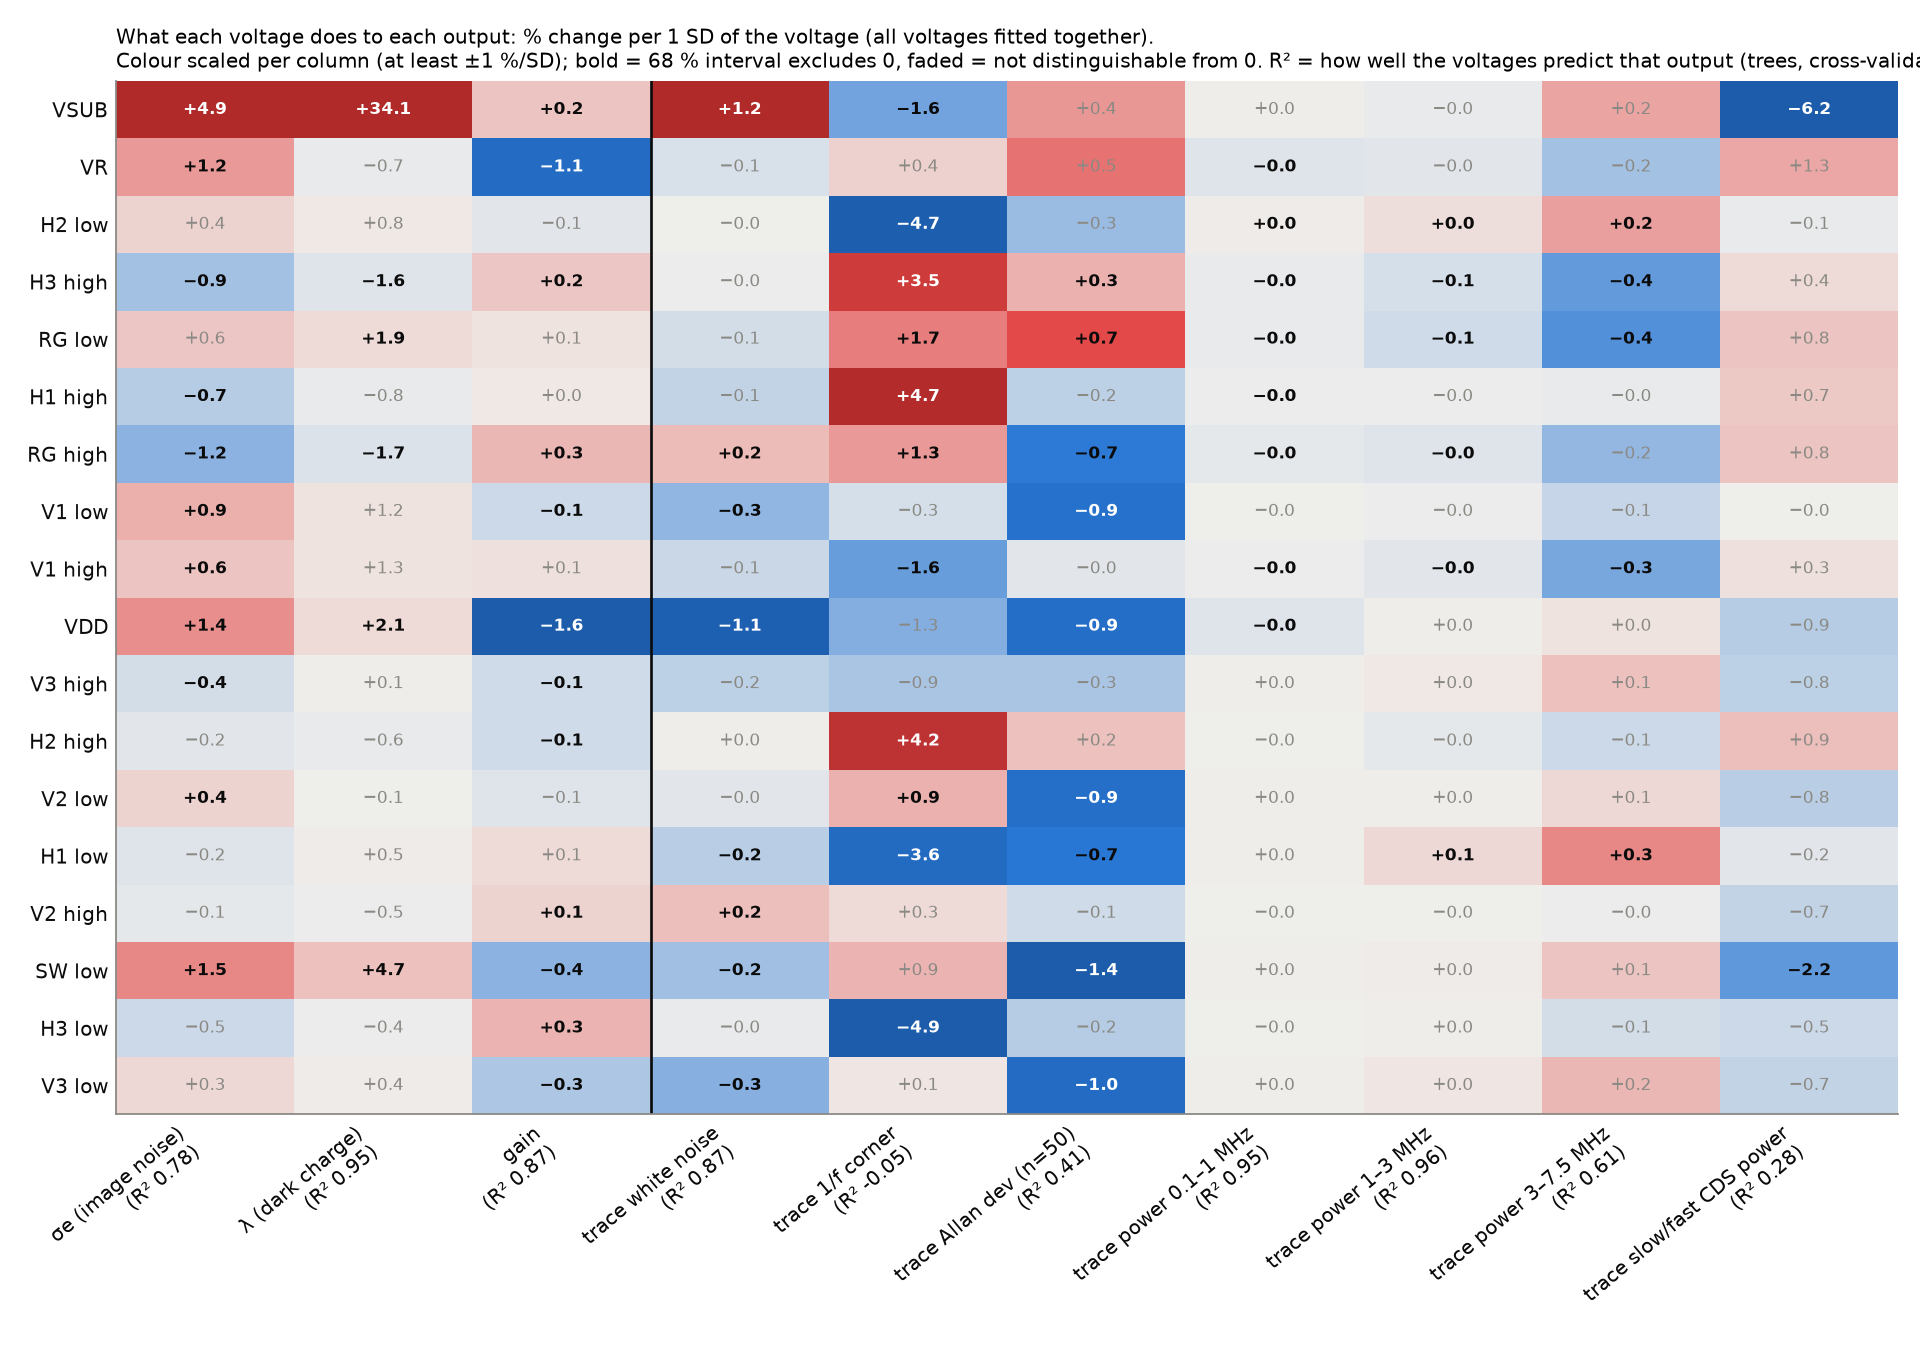
\includegraphics[width=\textwidth]{figures/effect_map.png}
\caption{The effect map: \% change of each output per 1~SD of each voltage, all voltages fitted together (session G,
232 measurements). Bold = the 68\,\% interval excludes zero. Columns left of the line are the image labels; right of
it the trace noise components. Colour is scaled per column.}\label{fig:effectmap}\end{figure}

\begin{table}[H]\centering\scriptsize
\caption{The five voltages that move each output most: \% change per 1~SD of the voltage (all voltages fitted together), and per volt in brackets. * = 68\% interval excludes zero. $R^2$: how well the voltages predict the output (cross-validated trees).}\label{tab:effects}
\begin{tabular}{p{2.6cm}cp{2.1cm}p{2.1cm}p{2.1cm}p{2.1cm}p{2.1cm}}\toprule
output & $R^2$ & 1st & 2nd & 3rd & 4th & 5th\\\midrule
$\sigma_e$ (image noise) & 0.78 & VSUB +4.9* (+0.5/V) & SW low +1.5* (+2.5/V) & VDD +1.4* (+1.4/V) & VR +1.2* (+2.4/V) & RG high $-$1.2* ($-$1.8/V)\\
$\lambda$ (dark charge) & 0.95 & VSUB +34.1* (+3.5/V) & SW low +4.7* (+7.8/V) & VDD +2.1* (+2.1/V) & RG low +1.9* (+1.8/V) & RG high $-$1.7* ($-$2.4/V)\\
gain & 0.87 & VDD $-$1.6* ($-$1.6/V) & VR $-$1.1* ($-$2.1/V) & SW low $-$0.4* ($-$0.7/V) & H3 low +0.3* (+0.6/V) & RG high +0.3* (+0.4/V)\\
trace white noise & 0.87 & VSUB +1.2* (+0.1/V) & VDD $-$1.1* ($-$1.1/V) & V3 low $-$0.3* ($-$2.1/V) & V1 low $-$0.3* ($-$1.9/V) & SW low $-$0.2* ($-$0.4/V)\\
trace 1/f corner & -0.05 & H3 low $-$4.9* ($-$11.4/V) & H1 high +4.7* (+10.0/V) & H2 low $-$4.7* ($-$10.6/V) & H2 high +4.2* (+10.7/V) & H1 low $-$3.6* ($-$8.5/V)\\
trace Allan dev (n=50) & 0.41 & SW low $-$1.4* ($-$2.4/V) & V3 low $-$1.0* ($-$6.7/V) & VDD $-$0.9* ($-$1.0/V) & V2 low $-$0.9* ($-$5.7/V) & V1 low $-$0.9* ($-$5.8/V)\\
trace power 0.1--1 MHz & 0.95 & VDD $-$0.0* ($-$0.0/V) & VR $-$0.0* ($-$0.1/V) & RG high $-$0.0* ($-$0.0/V) & RG low $-$0.0* ($-$0.0/V) & H3 high $-$0.0* ($-$0.0/V)\\
trace power 1--3 MHz & 0.96 & RG low $-$0.1* ($-$0.1/V) & H3 high $-$0.1* ($-$0.1/V) & H1 low +0.1* (+0.2/V) & H2 low +0.0* (+0.1/V) & RG high $-$0.0* ($-$0.1/V)\\
trace power 3--7.5 MHz & 0.61 & RG low $-$0.4* ($-$0.4/V) & H3 high $-$0.4* ($-$0.7/V) & H1 low +0.3* (+0.7/V) & V1 high $-$0.3* ($-$3.2/V) & H2 low +0.2* (+0.5/V)\\
trace slow/fast CDS power & 0.28 & VSUB $-$6.2* ($-$0.6/V) & SW low $-$2.2* ($-$3.6/V) & VR +1.3 (+2.5/V) & VDD $-$0.9 ($-$0.9/V) & H2 high +0.9 (+2.2/V)\\
\bottomrule\end{tabular}\end{table}



\subsection{Reading the effect map}
\begin{itemize}
\item \textbf{VSUB dominates both noise and dark charge.} $\lambda$ +34\,\%/SD (3.5\,\%/V; Sobol share 0.96), $\sigma_e$
  +4.9\,\%/SD (Sobol 0.66). It also raises the trace white noise (+1.2\,\%/SD) and lowers the slow/fast CDS power
  ratio ($-6.2$\,\%/SD), i.e.\ it adds fast (white) noise.
\item \textbf{After VSUB, for $\sigma_e$:} SW low +1.5, VDD +1.4, VR +1.2, RG high $-1.2$, V1 low +0.9, H3 high
  $-0.9$, H1 high $-0.7$\,\%/SD. Each is small (about one image's label noise) but they add up: together they are what
  is left when VSUB is held (Section~\ref{sec:subtle}).
\item \textbf{For $\lambda$ after VSUB:} SW low +4.7, VDD +2.1, RG low +1.9, RG high $-1.7$, H3 high $-1.6$\,\%/SD.
\item \textbf{Gain} is VDD ($-1.6$\,\%/SD, $-1.6$\,\%/V) and VR ($-1.1$\,\%/SD, $-2.1$\,\%/V); every other voltage
  $\le$0.4\,\%/SD.
\item \textbf{Trace white noise:} VSUB +1.2 and VDD $-1.1$\,\%/SD. In ADU, so the VDD part is mostly the gain:
  in electrons it nearly cancels.
\item \textbf{1/f corner:} the horizontal clocks (highs up, lows down = more swing $\to$ higher corner; about
  4--5\,\%/SD), but the corner is too noisy per trace to predict ($R^2\approx0$).
\item \textbf{Allan deviation at 50 skips (slow noise):} down about 1\,\%/SD with SW low, the V lows and VDD.
\item \textbf{Noise power in the 0.1--1, 1--3\,MHz bands:} essentially constant (well predicted, $R^2$ 0.95, but by the
  amplifier, not the voltages).
\end{itemize}

\takeaway{VSUB sets the dark charge and most of the noise. VDD and VR set the gain. Every other voltage moves
$\sigma_e$ by about 1--1.5\,\% per SD and $\lambda$ by 2--5\,\%, close to the measurement noise of one image. VSUB
raises $\sigma_e$ about four times more than it raises the trace's white noise, so most of its noise effect arises in the
image (through the dark charge), not in the amplifier.}

\subsection{Each amplifier}
\fig{effects_per_amp.png}{The six largest effects per label, for all amplifiers together (black, 68\,\% interval) and
for each amplifier (diamonds). The sign is the same on every amplifier; the size differs (VSUB on $\lambda$: ch0
+13\,\%, ch1 +43\,\%, ch3 +47\,\%/SD).}
The direction of every large effect is the same on all three amplifiers; the size is not. VSUB raises $\lambda$ three
times less on ch0 than on ch1 and ch3. This is the part a model can only learn from that amplifier's own data (or from its
traces).

\subsection{Shape: thresholds and knees}\label{sec:shape}
The linear effects hide where along a voltage the change happens:
\fig{partial_sigma_e.png}{$\sigma_e$ along its four strongest voltages, the others averaged out (one line per
amplifier). VSUB: flat to about 52\,V, then +13\,\% up to 70\,V. VR: switches on above $-2.8$\,V. H2 low: a jump at the
top of its window. H3 high: very low H highs (8.2--8.7\,V) add noise.}
\fig{partial_lambda.png}{$\lambda$ along its strongest voltages. VSUB is steep between 57 and 63\,V: median $\lambda$
0.20 at 35--42\,V, 0.73 at 66--71\,V.}
\fig{partial_gain.png}{Gain along its strongest voltages: smooth, nearly linear in VDD and VR.}
\fig{partial_white_noise.png}{Trace white noise along its strongest voltages.}

\subsection{Level against swing}\label{sec:swing}
Because each clock's high and low moved together, the effect map's ``high $+$, low $-$'' pattern on the 1/f corner is
better read as one effect of the \emph{swing}. Refitted with (low, swing = high $-$ low): H swing +7.5\,\%/SD and
V swing $-4.0$\,\%/SD on the 1/f corner; on $\sigma_e$, H swing $-1.1$\,\%/SD and V1 low +1.9\,\%/SD; on $\lambda$, V1 low
+3.3, V swing +1.8, H swing $-1.7$\,\%/SD.

% =====================================================================================================================
\section{Correlations}\label{sec:corr}
\subsection{Everything against everything}
The full matrix: 18 voltages, the three image labels and seven trace noise components, within an amplifier (each
quantity minus its amplifier mean). Faded numbers are not significant: with 80 packets, $|r|<0.22$.
\fig{corr_full.png}{All voltages, labels and trace noise components: Pearson correlation within amplifier (session G).
Top-left block = the design; the lines separate voltages, image labels and trace components.}
What it shows besides the voltage effects:
\begin{itemize}
\item $\sigma_e$ and $\lambda$ move together ($r=0.74$): both follow VSUB.
\item The trace white noise follows $\lambda$ (0.46) and $\sigma_e$ (0.32) and gain (0.38). It is the trace component
  closest to the image labels.
\item The slow/fast CDS power ratio falls with $\lambda$ ($-0.49$) and $\sigma_e$ ($-0.43$): more dark charge, more
  fast noise.
\item The 1--3 and 3--7.5\,MHz band powers are nearly the same measurement (0.94).
\end{itemize}
The rank (Spearman) version, robust to the VSUB knee and to outliers, gives the same picture
(\texttt{figures/corr\_full\_spearman.png}).

\subsection{Voltage against output: plain and ``this voltage alone''}
The left panel is the plain correlation; the right one is the \emph{partial} correlation, with every other voltage and
the amplifier held fixed. Where they differ, the plain correlation is borrowed from another voltage.
\fig{corr_knobs_outputs.png}{Voltage vs output. Left: plain correlation within amplifier. Right: partial correlation
(this voltage alone). Faded = not significant.}
\textbf{The plain correlations mislead for the clock rails.} V1 low (0.37), V3 low (0.29), V2 low (0.22), H3 high
($-0.36$) and H3 low ($-0.35$) all look correlated with $\sigma_e$, and similarly with $\lambda$; held against the other
voltages they fall to $\le0.11$. They were correlated with VSUB in the design (relational rules), and VSUB does the
work. Alone, only VSUB (0.54), VDD (0.20), RG high ($-0.17$), VR (0.16) and SW low (0.15) relate to $\sigma_e$, and only
VSUB (0.84) clearly to $\lambda$. This is why every effect in Section~\ref{sec:effects} is fitted with all voltages at
once.

\begin{table}[H]\centering\scriptsize
\caption{The five voltages most correlated with each output \emph{on their own} (partial correlation: the other voltages and the amplifier held fixed), with the plain within-amplifier correlation in brackets. * = significant ($|r|\ge0.22$).}\label{tab:corr}
\begin{tabular}{p{3cm}p{2.2cm}p{2.2cm}p{2.2cm}p{2.2cm}p{2.2cm}}\toprule
output & 1st & 2nd & 3rd & 4th & 5th\\\midrule
$\sigma_e$ (noise) & VSUB +0.55* (+0.63) & VDD +0.20 ($-$0.04) & RG high $-$0.17 ($-$0.06) & VR +0.16 (+0.17) & SW low +0.15 ($-$0.21)\\
$\lambda$ (dark charge) & VSUB +0.84* (+0.88) & SW low +0.16 ($-$0.18) & VDD +0.10 ($-$0.20) & RG low +0.09 (+0.13) & V3 high +0.09 (+0.02)\\
gain & VDD $-$0.75* ($-$0.63) & VR $-$0.58* ($-$0.40) & SW low $-$0.20 (+0.10) & RG high +0.18 ($-$0.20) & H2 low +0.15 (+0.07)\\
trace: white noise & VDD $-$0.51* ($-$0.54) & VSUB +0.50* (+0.55) & H3 low +0.09 ($-$0.10) & RG high +0.09 ($-$0.01) & SW low $-$0.09 ($-$0.03)\\
trace: 1/f corner & RG low +0.09 (+0.03) & VSUB $-$0.08 ($-$0.02) & VDD $-$0.08 ($-$0.01) & RG high +0.07 (+0.01) & V1 high $-$0.05 ($-$0.03)\\
trace: Allan dev n=50 & SW low $-$0.12 ($-$0.01) & VDD $-$0.11 ($-$0.12) & RG high $-$0.08 ($-$0.08) & RG low +0.08 (+0.06) & V3 low +0.07 ($-$0.06)\\
trace: power 0.1-1 MHz & VDD $-$0.29* ($-$0.29) & VR $-$0.24* ($-$0.28) & RG high $-$0.18 ($-$0.28) & RG low $-$0.13 ($-$0.06) & V1 low +0.10 (+0.00)\\
trace: power 1-3 MHz & RG low $-$0.25* ($-$0.23) & RG high $-$0.13 ($-$0.09) & VR $-$0.11 ($-$0.11) & V1 low +0.11 ($-$0.04) & H2 low +0.09 (+0.06)\\
trace: power 3-7.5 MHz & RG low $-$0.21 ($-$0.18) & RG high $-$0.12 ($-$0.09) & VSUB +0.12 (+0.14) & V1 low +0.10 ($-$0.01) & VR $-$0.10 ($-$0.06)\\
trace: slow/fast CDS power & VSUB $-$0.42* ($-$0.43) & SW low $-$0.12 (+0.05) & V1 low $-$0.10 ($-$0.09) & VR +0.10 (+0.03) & H1 low $-$0.09 (+0.06)\\
\bottomrule\end{tabular}\end{table}



\subsection{Each amplifier}
\fig{corr_per_amp.png}{Voltage vs output correlation per amplifier (plain, not within-amplifier, since each panel is one
amplifier).}

% =====================================================================================================================
\section{How well the models predict}\label{sec:models}
All models of the level-1 scorecard were trained and scored on session G with cross-validation: five time blocks, and
for ``new amplifier'' each amplifier left out in turn. Trace models never see the settings. The absolute models answer
``what is $\sigma_e$ at this setting?''; the change models answer ``how much does $\sigma_e$ change from setting A to
setting B on the same amplifier?''. Appendix~\ref{app:models} describes each model.

\subsection{Absolute models}
\fig{models_absolute.png}{Absolute models: typical error (\%) per label. Top: amplifiers seen in training; bottom: a
new amplifier. Dark blue $\bigstar$ = frozen top three; gray = baselines (predict the mean, or each amplifier's mean);
orange diamonds = the sealed session H.}
\begin{itemize}
\item \textbf{Trained amplifiers:} settings + amplifier identity is best for $\lambda$ (11\,\% vs 55\,\% for the
  mean) and gain (0.8\,\% vs 3.1\,\%). For $\sigma_e$, the trace physics model, settings + amplifier trees and trace
  trees tie at 6.3--6.5\,\% (vs 13.8\,\%).
\item \textbf{New amplifier:} the settings alone hardly beat the mean ($\sigma_e$ 17.7 vs 18.2\,\%, $\lambda$ 64--67
  vs 70\,\%), because most of the variation is between amplifiers. The traces carry the amplifier: trace trees give
  $\sigma_e$ 11.9\,\% and $\lambda$ 40\,\%. For gain, the settings stay best (3.7\,\%).
\item The flexible trace models (NN, CNN, pretrained CNN, deep kernel GP) do worse than the trees on a new amplifier:
  with 80 packets they overfit.
\end{itemize}
\fig{scatter_absolute.png}{Predicted vs measured for the frozen \#1 absolute model per label and cell (session G,
cross-validated).}

\subsection{Change models}
\fig{models_change.png}{Change models: size error (\%) of the predicted change, random pairs of packets, with the rank
correlation $\rho$. Gray = predicting no change. Dark blue $\bigstar$ = frozen top three; orange = session H.}
\begin{itemize}
\item \textbf{$\lambda$ and gain are a ``settings'' problem.} On a new amplifier the settings change models rank the
  $\lambda$ changes with $\rho=0.86$--0.87 and gain with 0.77--0.78; trace-only models reach 0.66--0.74 and 0.61--0.69.
  Adding the traces to the settings (settings + trace combined trees) cuts the $\lambda$ error from 36\,\% to 25\,\%
  ($\rho$ 0.93).
\item \textbf{$\sigma_e$ is hard for every model.} On a new amplifier the best reach $\rho\approx0.6$--0.67 and cut the
  error from 11.9\,\% (no change) to 9.3\,\%. Traces are as good as or slightly better than the settings here.
\item \textbf{On trained amplifiers} settings + traces is best everywhere: $\rho$ 0.78 ($\sigma_e$), 0.96 ($\lambda$),
  0.91 (gain).
\end{itemize}
\fig{scatter_change.png}{Predicted vs true change for the frozen \#1 change model (gray: random pairs; blue: the
nominal reference and the new setting of the same packet). For $\lambda$ on a new amplifier, the blue cluster that sits
too high (true +30\,\%, predicted +100\,\%) is one amplifier (ch0), whose VSUB response is three times weaker.}

\subsection{The physics model}
The physics model predicts $\sigma_e$ from the trace's measured noise (white and 1/f, passed through the CDS filter)
and the gain; the ``difference'' version applies it to the change between two traces, and ``+ correction'' adds trees
that learn what the physics misses. It needs no settings and has few free parameters, so it is the reference that
should carry over to new hardware.
\fig{physics.png}{The physics model. Left two: absolute $\sigma_e$ (trained amplifiers 6.3\,\%, new amplifier 14.0\,\%).
Right: its change versions on a new amplifier; the pure difference ($\rho$ 0.39) misses the image part of the noise (the
VSUB/dark-charge part); the correction brings it to $\rho$ 0.63.}
The physics model is the best absolute $\sigma_e$ model on trained amplifiers (6.3\,\%) and second on a new amplifier
(14.0\,\%, after the trace trees). As a change model it is weak on its own ($\rho$ 0.38--0.39): the trace sees the
amplifier noise, while most of what VSUB does to $\sigma_e$ arises in the image.

% =====================================================================================================================
\section{Can the models see the small effects?}\label{sec:subtle}
Every v3 packet moves every voltage, so the change between two packets is dominated by VSUB (for $\sigma_e$ and
$\lambda$) or VDD and VR (for gain). To test the small effects, take the pairs where the dominant knob moved by less than
0.25~SD (VSUB within 2.4\,V); what remains is the sum of the small effects of all other voltages.
\fig{subtle.png}{Rank correlation of predicted vs true change for all scored pairs and for pairs where the dominant knob
barely moved. Settings only (light blue), traces only (orange), settings + traces (dark blue).}
\begin{table}[H]\centering\scriptsize
\caption{Small effects: rank correlation $\rho$ of predicted vs true change (size error \% in brackets), all scored pairs against pairs where the dominant knob moved $<0.25$~SD. True RMS = how big the true changes are.}\label{tab:subtle}
\begin{tabular}{lllr rlllll}\toprule
cell & label & pairs & n & true RMS & settings & traces & traces (ens.) & settings + traces & settings + traces (ens.)\\\midrule
trained & noise $\sigma_e$ & all pairs & 2291 & 12.0\% & 0.69 (9.6) & 0.69 (9.2) & 0.73 (8.5) & 0.79 (8.0) & 0.79 (7.9)\\
trained & noise $\sigma_e$ & VSUB held & 532 & 8.4\% & 0.50 (6.7) & 0.51 (6.6) & 0.53 (6.3) & 0.57 (6.1) & 0.58 (6.0)\\
trained & dark charge $\lambda$ & all pairs & 2291 & 53.5\% & 0.91 (27.5) & 0.77 (32.2) & 0.83 (27.3) & 0.97 (13.8) & 0.95 (17.7)\\
trained & dark charge $\lambda$ & VSUB held & 532 & 30.6\% & 0.73 (15.7) & 0.30 (19.7) & 0.38 (17.5) & 0.76 (10.1) & 0.71 (11.0)\\
trained & gain & all pairs & 2291 & 3.1\% & 0.81 (1.9) & 0.77 (2.2) & 0.83 (1.9) & 0.91 (1.4) & 0.90 (1.4)\\
trained & gain & VDD and VR held & 242 & 2.3\% & 0.84 (1.3) & 0.79 (1.6) & 0.80 (1.6) & 0.89 (1.0) & 0.86 (1.1)\\
new amp & noise $\sigma_e$ & all pairs & 2291 & 12.0\% & 0.61 (10.7) & 0.65 (10.2) & 0.66 (9.4) & 0.65 (10.5) & 0.68 (9.3)\\
new amp & noise $\sigma_e$ & VSUB held & 532 & 8.4\% & 0.43 (7.3) & 0.49 (7.1) & 0.50 (6.7) & 0.54 (7.5) & 0.54 (6.5)\\
new amp & dark charge $\lambda$ & all pairs & 2291 & 53.5\% & 0.88 (35.8) & 0.73 (36.1) & 0.73 (33.8) & 0.94 (24.9) & 0.91 (25.2)\\
new amp & dark charge $\lambda$ & VSUB held & 532 & 30.6\% & 0.71 (20.3) & 0.32 (22.4) & 0.29 (20.3) & 0.74 (15.8) & 0.64 (16.8)\\
new amp & gain & all pairs & 2291 & 3.1\% & 0.77 (2.2) & 0.71 (2.4) & 0.69 (2.5) & 0.78 (2.3) & 0.78 (2.3)\\
new amp & gain & VDD and VR held & 242 & 2.3\% & 0.80 (1.6) & 0.73 (1.8) & 0.71 (1.7) & 0.80 (1.6) & 0.79 (1.6)\\
\bottomrule\end{tabular}\end{table}


\begin{itemize}
\item \textbf{$\sigma_e$ with VSUB held:} the true changes are still 8.4\,\% RMS (label noise 1.9\,\%). On a new
  amplifier the settings rank them with $\rho=0.43$, the traces with 0.49--0.50, both together 0.54. The small
  noise effects \emph{are} seen, partly, and slightly better from the traces than from the settings.
\item \textbf{$\lambda$ with VSUB held:} the settings keep $\rho=0.71$; the traces fall to 0.29--0.32. The small
  dark-charge effects (SW low, VDD, RG) are visible from the settings but not in a 0.2\,s trace.
\item \textbf{Gain with VDD and VR held:} both still work ($\rho$ 0.73--0.80).
\end{itemize}
\takeaway{The settings alone pick up the small voltage effects on $\lambda$ and gain. For $\sigma_e$ the small effects
are only half captured by anything; the traces see them a bit better than the settings, and the two together best.}

% =====================================================================================================================
\section{Frozen model choice and the sealed test}\label{sec:frozen}
Before session H was opened, the top three models per label were frozen
(\texttt{lvl1/frozen\_choice\_v3.json}), separately for absolute and change models, and for trained amplifiers and a new
amplifier: absolute by typical error, change by size error on random pairs. The physics models, the settings
references and the baselines were always kept. Session H (24 new settings + 5 nominal, 67 measurements) was then scored
once, with every model trained on all of session G.
\begin{table}[H]\centering\scriptsize
\caption{The frozen top three absolute models per target (typical error \%): session G (cross-validated, used to choose) $\to$ sealed session H (scored once). Lower is better.}
\begin{tabular}{llp{4cm}p{4cm}p{4cm}}\toprule
cell & target & 1st & 2nd & 3rd\\\midrule
trained amps & noise $\sigma_e$ & trace: physics: 6.3 $\to$ 7.6 & settings + amplifier: trees: 6.4 $\to$ 7.7 & trace: trees: 6.5 $\to$ 8.0\\
trained amps & dark charge $\lambda$ & settings + amplifier: gp: 11.1 $\to$ 14.6 & settings + amplifier: trees: 11.9 $\to$ 10.5 & trace: trees: 20.6 $\to$ 26.1\\
trained amps & gain & settings + amplifier: gp: 0.8 $\to$ 0.6 & settings + amplifier: trees: 1.0 $\to$ 0.9 & trace: physics: 1.1 $\to$ 1.1\\
new amp & noise $\sigma_e$ & trace: trees: 11.9 $\to$ 12.7 & trace: physics: 14.0 $\to$ 13.5 & trace: nn: 15.3 $\to$ 14.2\\
new amp & dark charge $\lambda$ & trace: trees: 39.9 $\to$ 49.5 & trace: physics: 51.5 $\to$ 50.9 & trace: nn: 57.2 $\to$ 51.1\\
new amp & gain & settings: trees: 3.7 $\to$ 3.6 & settings: gp: 3.7 $\to$ 3.9 & trace: physics: 4.0 $\to$ 4.3\\
\bottomrule\end{tabular}\end{table}

\begin{table}[H]\centering\scriptsize
\caption{The frozen top three change models per target (size error \% (random pairs)): session G (cross-validated, used to choose) $\to$ sealed session H (scored once). Lower is better.}
\begin{tabular}{llp{4cm}p{4cm}p{4cm}}\toprule
cell & target & 1st & 2nd & 3rd\\\midrule
trained amps & noise $\sigma_e$ & ensemble: settings + trace: 8.0 $\to$ 10.0 & settings + trace: combined trees: 8.1 $\to$ 11.4 & ensemble: trace models: 8.5 $\to$ 10.3\\
trained amps & dark charge $\lambda$ & settings + trace: combined trees: 14.0 $\to$ 15.3 & absolute settings + amplifier: gp, differenced: 14.4 $\to$ 19.3 & absolute settings + amplifier: trees, differenced: 16.4 $\to$ 14.6\\
trained amps & gain & absolute settings + amplifier: gp, differenced: 1.0 $\to$ 0.8 & absolute settings + amplifier: trees, differenced: 1.4 $\to$ 1.3 & settings + trace: combined trees: 1.4 $\to$ 0.9\\
new amp & noise $\sigma_e$ & ensemble: settings + trace: 9.3 $\to$ 11.2 & ensemble: trace models: 9.4 $\to$ 11.5 & trace change: difference curves PCA + trees: 9.7 $\to$ 14.2\\
new amp & dark charge $\lambda$ & ensemble: settings + trace: 25.3 $\to$ 34.3 & settings + trace: combined trees: 25.3 $\to$ 29.9 & settings + trace: residual trees: 32.6 $\to$ 33.5\\
new amp & gain & settings change: gp: 2.3 $\to$ 1.9 & settings change: trees: 2.3 $\to$ 1.8 & ensemble: settings + trace: 2.3 $\to$ 2.1\\
\bottomrule\end{tabular}\end{table}



\subsection{Results on session H}
Session H was scored once (67 measurements, 24 new settings; ``new amplifier'' = trained without that amplifier).
H's changes are bigger than G's (predicting no change: $\sigma_e$ 14.0\,\% against 11.9\,\%, $\lambda$ 63.5 against
53.8\,\%), so read the rank correlation $\rho$ first.

\begin{table}[H]\centering\small
\caption{Frozen change models, random pairs: size error \% and $\rho$, session G (cross-validated) $\to$ sealed session H.}
\begin{tabular}{llll}\toprule
label, cell & model & size error & $\rho$\\\midrule
$\sigma_e$, new amp & ensemble: settings + trace & 9.3 $\to$ 11.2 & 0.67 $\to$ 0.73\\
 & ensemble: trace models & 9.4 $\to$ 11.5 & 0.65 $\to$ 0.63\\
 & trace change: difference curves PCA + trees & 9.7 $\to$ 14.2 & 0.59 $\to$ 0.46\\
 & (settings change: trees, reference) & 10.9 $\to$ 12.9 & 0.60 $\to$ 0.64\\
 & (physics difference + correction) & 10.3 $\to$ 11.5 & 0.63 $\to$ 0.65\\
$\lambda$, new amp & settings + trace: combined trees & 25.3 $\to$ 29.9 & 0.93 $\to$ 0.94\\
 & ensemble: settings + trace & 25.3 $\to$ 34.3 & 0.91 $\to$ 0.91\\
 & settings + trace: residual trees & 32.6 $\to$ 33.5 & 0.89 $\to$ 0.91\\
 & (settings change: trees) & 36.4 $\to$ 38.9 & 0.87 $\to$ 0.89\\
gain, new amp & settings change: gp / trees & 2.3 $\to$ 1.8--1.9 & 0.78 $\to$ 0.87\\
 & ensemble: settings + trace & 2.3 $\to$ 2.1 & 0.78 $\to$ 0.87\\
$\sigma_e$, trained & ensemble: settings + trace & 8.0 $\to$ 10.0 & 0.78 $\to$ 0.82\\
$\lambda$, trained & settings + trace: combined trees & 14.0 $\to$ 15.3 & 0.96 $\to$ 0.98\\
gain, trained & absolute settings + amplifier GP, differenced & 1.0 $\to$ 0.8 & 0.95 $\to$ 0.97\\\bottomrule
\end{tabular}\end{table}
Absolute models on H: settings + amplifier $\lambda$ 10.5--14.6\,\% (G 11.1--11.9), gain 0.6--0.9\,\% (G 0.8--1.0);
trace physics $\sigma_e$ 7.6\,\% trained, 13.5\,\% new (G 6.3, 14.0); trace trees $\lambda$ on a new amplifier 49.5\,\%
(G 39.9: the one absolute choice that degraded).
\takeaway{The choice made on session G holds on new settings: the settings + trace models are the best change models
for every label, the settings alone for gain on a new amplifier. The pure trace-difference models are the least
stable.}


% =====================================================================================================================
\section{Choosing a setting}
For each setting, the score is the board's mean over the three amplifiers of $w\,\Delta\log\sigma_e + (1-w)\,\Delta\log
\lambda$. Each model shortlists five settings; the regret is how much worse the best of those five truly is than the
truly best of the 60 session-G settings.
\begin{itemize}
\item \textbf{Settings models} (alone, with the amplifier or with traces) put the truly best setting on the shortlist at
  every weighting, with 0--1\,\% regret, on trained and new amplifiers.
\item \textbf{Trace-only models} manage that only when $\sigma_e$ is all that counts ($w=1$); as soon as $\lambda$
  counts, their regret is 3--12\,\% (random choice: 8--31\,\%).
\end{itemize}
Because VSUB dominates both outputs, ``lowest VSUB'' is close to the right answer, and every model that knows VSUB finds
it.

% =====================================================================================================================
\section{Conclusions}
\begin{enumerate}
\item For a fixed timing, \textbf{VSUB is the knob} for both noise and dark charge; keep it below the 55--60\,V knee
  unless depletion needs more. VDD and VR are the gain knobs. Everything else is a 1--5\,\% effect.
\item To predict a \textbf{change on a known amplifier}, use settings + traces (combined trees, or the ensemble): $\rho$
  0.8 ($\sigma_e$), 0.98 ($\lambda$), 0.97 (gain) on new settings.
\item On a \textbf{new amplifier}, the settings carry $\lambda$ and gain ($\rho$ 0.87--0.94); for $\sigma_e$ every
  model is limited ($\rho\approx0.6$--0.7) because a large part of the noise change happens in the image (charge), not in
  the amplifier the trace sees, and because the readout chain's own noise dominates each skip (amp\_phys report).
\item The physics model is a robust $\sigma_e$ reference (stable G $\to$ H) but needs its correction trees for changes.
\item Next: the amplifier-physics datasheet (folder \texttt{amp\_phys}) explains the amplifier differences the models
  have to learn (101 ch2: a telegraph-noise trap; ch0/ch2: weak VSUB response on the register side).
\end{enumerate}


% =====================================================================================================================
\appendix
\section{The models}\label{app:models}
\begin{description}
\item[settings: gp / trees] the voltages only; a Gaussian process or boosted trees. Knows nothing of the amplifier.
\item[settings + amplifier] the same with the amplifier's identity as input; only possible on amplifiers seen in
  training.
\item[trace: physics] $\sigma_e$ from the trace's fitted white and 1/f noise through the CDS filter, divided by the
  gain; $\lambda$ and gain from a small hierarchical fit on trace features.
\item[trace: trees / gp / nn / cnn / pretrained cnn / deep kernel] the trace features (or the raw spectrum, for the CNNs)
  into boosted trees, a GP, a small network, a 1-D CNN (from scratch or pretrained on v2) or a GP on network features.
\item[settings change: gp / trees] the change of every voltage (B $-$ A) and the starting voltages $\to$ the change.
\item[trace change: trees] the change of every trace feature $\to$ the change.
\item[trace: combined trees {[A, B, B$-$A]}] both traces' features and their difference $\to$ the change.
\item[trace change: shared-encoder net] one network encodes each trace; the difference of the encodings $\to$ the
  change.
\item[trace change: difference curves PCA + trees / hand-picked bands + gp] the difference of the two noise spectra,
  compressed by PCA or summed over hand-picked bands.
\item[trace: physics difference (+ correction)] the physics $\sigma_e$ of B minus that of A (+ trees on the trace
  features for what it misses).
\item[settings + trace: combined trees] settings change and trace features together.
\item[settings + trace: residual trees] the settings change model, corrected by trees on the trace features.
\item[direction classifiers] only up or down, not how much.
\item[absolute \dots, differenced] an absolute model applied to A and B, subtracted.
\item[ensembles] the average of: trace change trees, trace combined trees, physics difference + correction and the
  differenced physics model (trace models); settings + trace combined and residual trees and the two physics ones
  (settings + trace).
\end{description}

\section{Files}
\begin{itemize}
\item Scorecards: \texttt{processed\_v3n/lvl1\_results/scorecard\_G}, \texttt{scorecard\_H} (\texttt{scorecard.md} has
  every pair type and every metric).
\item Effects: \texttt{processed\_v3n/lvl1\_results/parameter\_influence\_noise/influence.md} (all knobs, Sobol, per
  amplifier, level vs swing).
\item Correlations: \texttt{processed\_v3n/lvl1\_results/correlations} (CSV of every matrix).
\item Small effects: \texttt{processed\_v3n/lvl1\_results/subtle}.
\item Scripts: \texttt{lvl1/parameter\_influence.py}, \texttt{correlation\_v3.py}, \texttt{subtle\_v3.py},
  \texttt{freeze\_choice\_v3.py}, \texttt{report\_v3.py}, \texttt{scorecard\_v2.py}, \texttt{reconstruct\_records.py}.
\end{itemize}
\end{document}
